% Comparison of the techniques presented
\section{Analysis of techniques}
\label{sec:technique}
Reconfiguration capabilities and hardware-software codesign techniques are elements of a complex scenario. In this section we will discuss and analyze these capabilities and techniques seperately. To create such a self-adaptive autonomic system, the system has to be self-aware, able to make decisions, self-adapting and the hardware has to support a certain amount of reconfiguration. In section \ref{sec:proposition} the overall best combination will be presented, utlizing the flexibility of software and the speed of hardware.

%-----------------------------------------------------------------------------------------

\subsection{Monitoring techniques}
\label{sec:selfawareness}
The heartbeats application as discussed in section \cite{sec:selfaware} is a technique used for monitoring. A framework like this is particularly convenient because it allows to automatically update all information about the global heart-rate which is then made available to external observers, such as decision making applcations. However it introduces an average overhead of 3,52\% due to system calls in order to initialize its data structures and updating the global heart rate \cite{selfaware}.
\subsection{Decision making techniques}
\label{sec:decisions}

* present heuristics, best algorithm etc *
\subsection{Self-adapting techniques}
\label{sec:selfadapting}

A self-aware adaptive computing system is an active system where the hardware, the applications and the operating system have to be seen as an unique entity that can autonomously adapt itself to achieve the best performance. \cite{selfaware} presents a general overview of the hardware and software architecture components of a self-aware computing system as can be seen in figure \ref{fig:selfaware}. Cognitive hardware mechanisms available in the underlying hardware \emph{observe} and \emph{affect} the exectution. 

% -- Plaatje self-aware hardware and software architecture---------------------------
\begin{figure}[htb]%
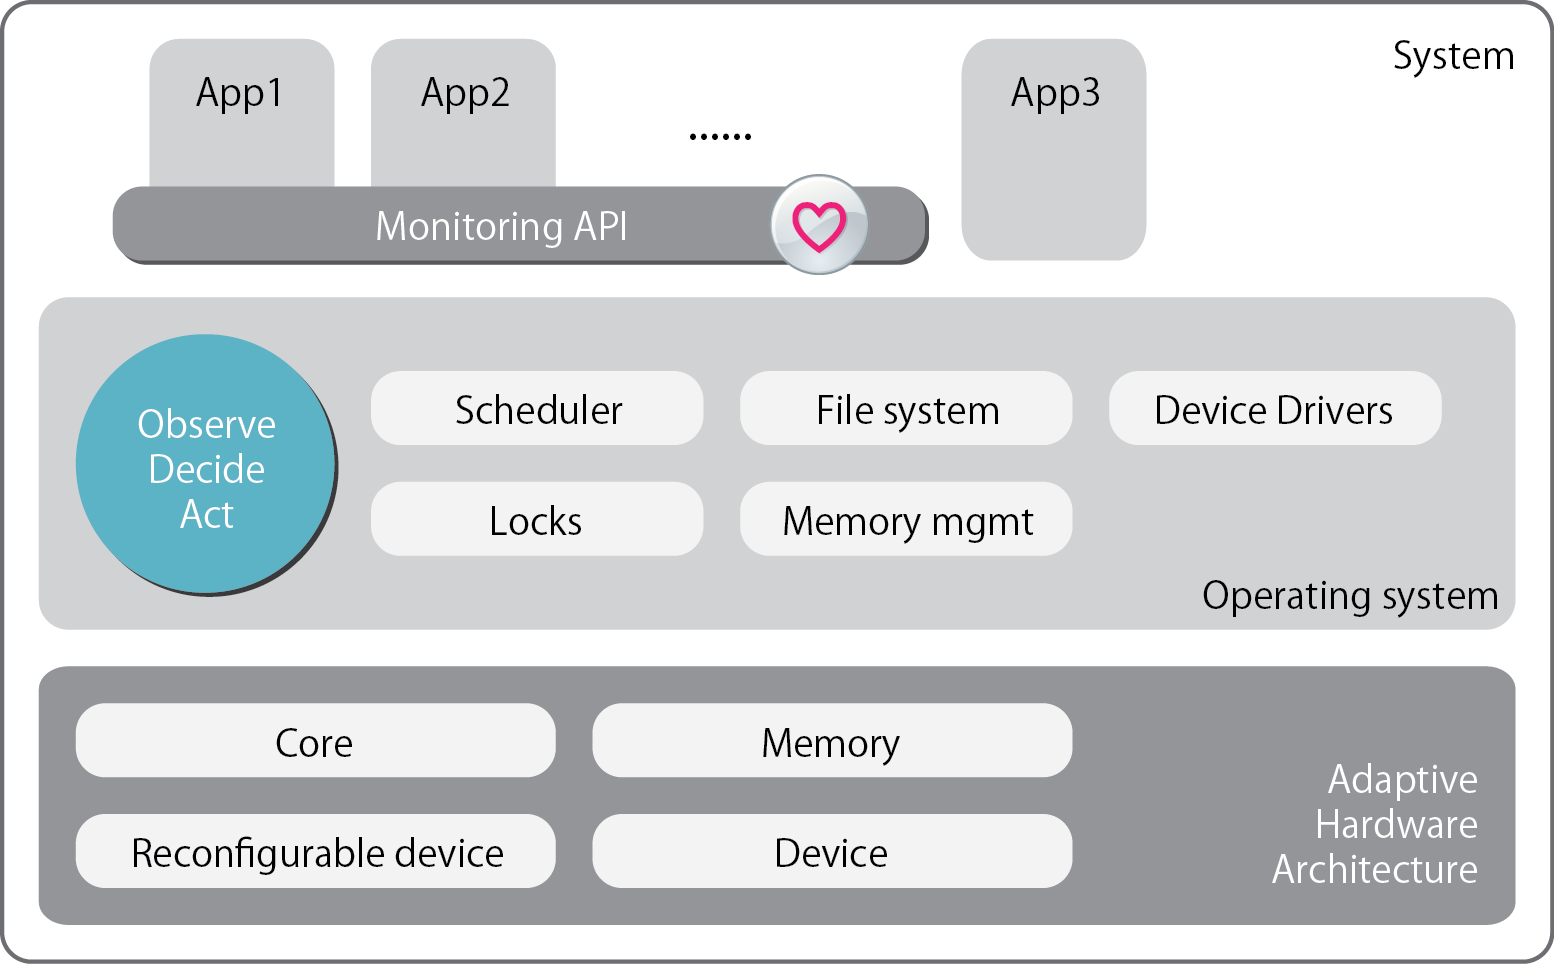
\includegraphics[width=\columnwidth]{Pictures/self-aware.PNG}%
\caption{Overview of the proposed self-aware adaptive FPGA-based computing system presented in \cite{selfaware}}%
\label{fig:selfaware}%
\end{figure}
%------------------------------------------------------------------------------------------------
A fundamental part of a self-aware adaptive computing system is the ability to switch between implementations of the same functionality while the system is running. A control system has to be developed as an actuator in the oberserve-decide-act loop. The \emph{hot-swap mechanism} is a popular tool to inplement self-configuration and self-optimization. Although it provides the ability of switching among different implementations of the same functionality in a transparent fashion, state quiescence and state translation are two big issues when using this mechanism and need a framework solution to be reliable. 

Other works present \emph{Partial Dynamic Reconfiguration (PDR)} \cite{reconfigurable} to reduce the amount of overhead introduced by reconfiguration. Hardware portions can adapt over time to cope with new requirements creating an adaptive system. If the application can be partitioned into different phases, PDR can configure the modules one after another to keep area requirements lower than having all functionalities loaded at the same time. PDR can thus be seen as a trade-off between the speed of hardware and the flexibility of software.  
% Discussion of different hardware techniques
% Aimee, 1 nov 2013

\subsubsection{Virtex FPGA with a Two-Dimensional Reconfiguration Core}
\label{sec:fpga}
On Virtex-4 FPGAs, two-dimensional dynamic reconfiguration like figure \ref{fig:2d} is supported. With 2D reconfiguration it becomes possible to reconfigure device portions whose height is not constrained to be the device height. This architecture of the reconfiguration core (or RC) speeds up the reconfiguration time and thus the evolution time.  The RC can also deploy more candidate solutions as discussed in \cite{virtex4}, which are arrays of bidimensional cell (see figure \ref{fig:candidate}). An alternative for candidate solutions is a mesh-type systolic array of parallel processing elements (PEs) from \cite{dpr}, also following a 2D architecture for the RC. A major feature is the possibility to change the functionality of the PEs by means of Dynamic and Partial Reconfiguration (DPR). This gives the system the capability to adapt. The outputs of the PEs (east and south side) are connected to the close neighbour's input (west and north side), such that only the lowest and right-most PE has to be read for data output. This systolic approach of communication reduces the reconfiguration time and makes the architecture easy to extend.

A drawback of using Virtex FPGAs are the feed-through signales, mentioned in \cite{erlangen}. Each module must be implemented with all possible feed-through channels  needed by other modules. Because we only know at run-time which module needs to feed through a signal, many channels reserved for a possible feed-through become redundant. Also, modules accessing external pins are no longer relocatable, because they are complied for fixed locations where a direct signal line to these pins is established.

% -- Plaatje 2D RC architecture ---------------------------
\begin{figure}[htb]%
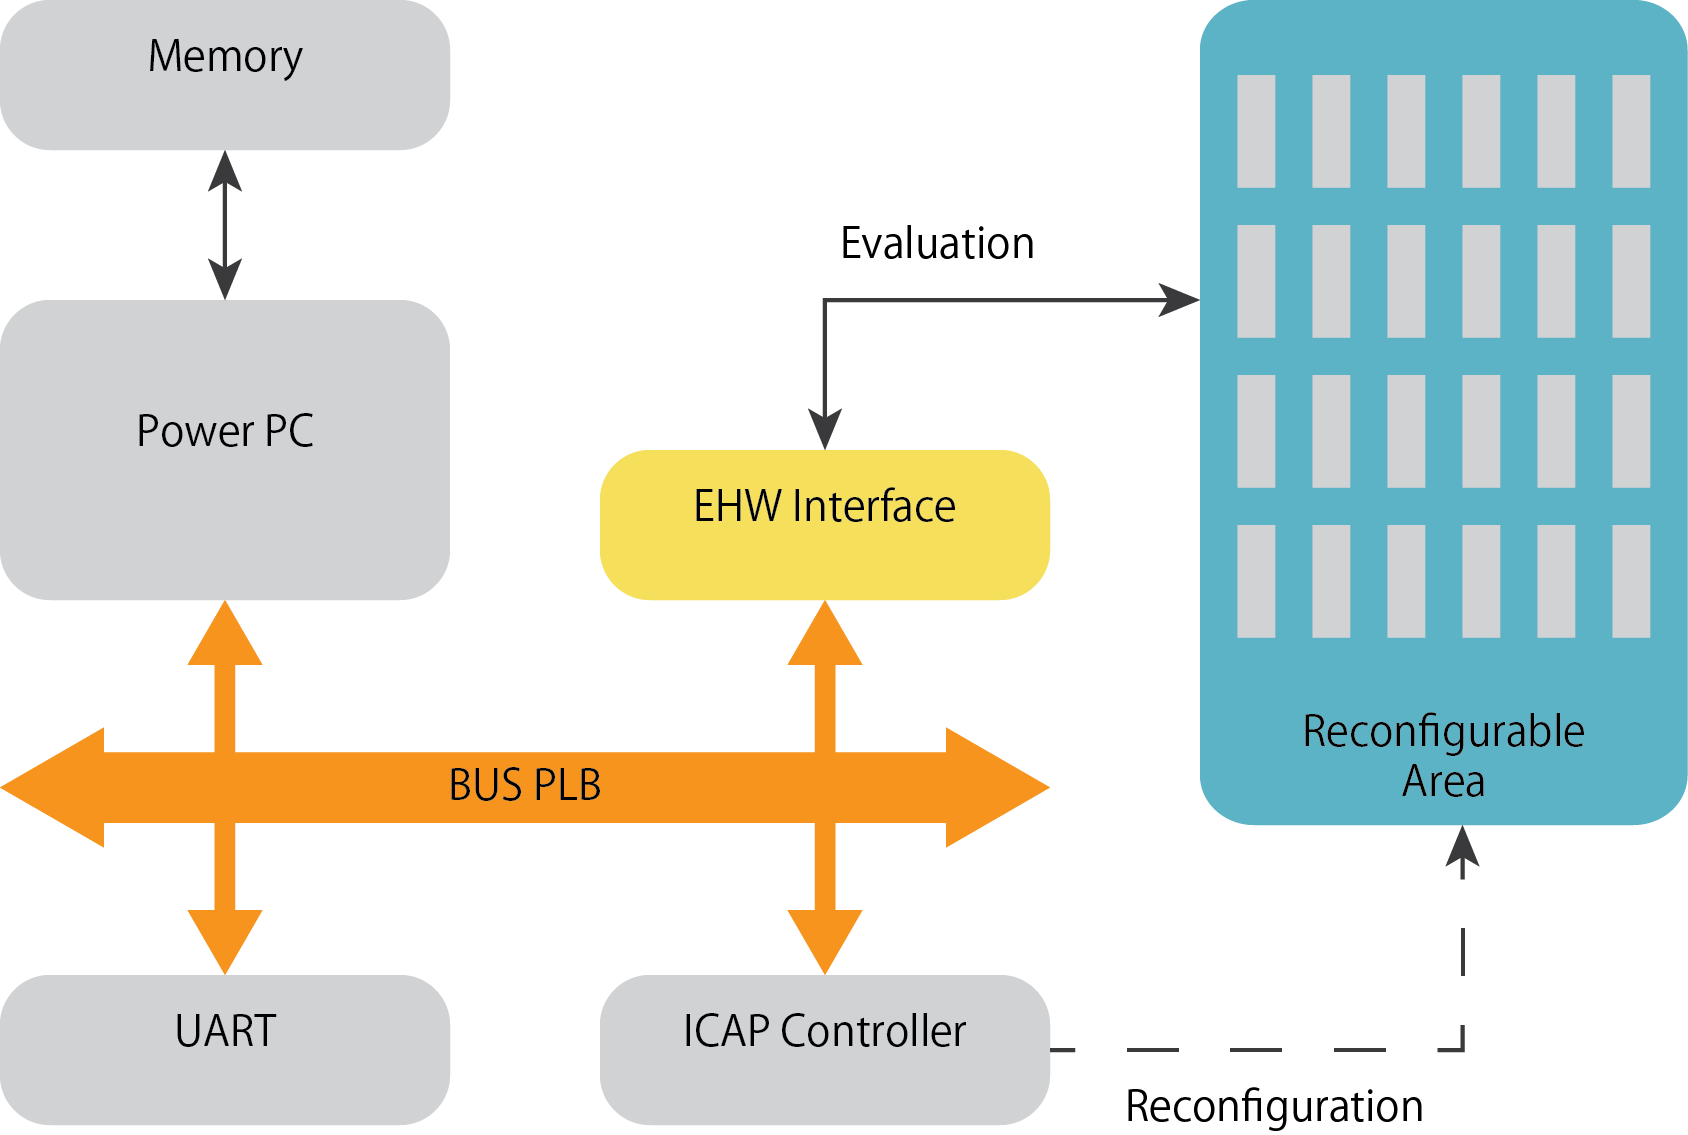
\includegraphics[width=\columnwidth]{Pictures/2D_architecture.png}%
\caption{High-level structure of a Two-Dimensional Architecture depicted in \cite{virtex4}}%
\label{fig:2d}%
\end{figure}

\subsubsection{Candidate Solutions and Direct Bitstream Manipulation}

With a 2D architecture for the RC, \cite{virtex4} uses safe manipulation of the bitstream to overcome the unknown and undocumented bitstream mentioned in \ref{sec:virtex4}. Candidate solutions are used to fill the RC with cells, which have an internal flip-flops allowing the evolution of synchronous circuits. This is a common structure for evolvable hardware (EHW) systems making use of direct bitstream manipulation \cite{virtex4}. For the cell structure of the candidate solutions the use of LUTs and a MUX is proposed, in order to provide direct bitstream manipulation. Combined with the 2D-reconfiguration mechanism, the new architecture causes a speed up of 16x factor. For this system, only Virtex-4 or Virtex-5 FPGAs can be used since Virtex-II does not support 2D reconfiguation (\cite{virtex4}.

% -- Plaatje candidate solutions architecture ---------------------------
\begin{figure}[htb]%
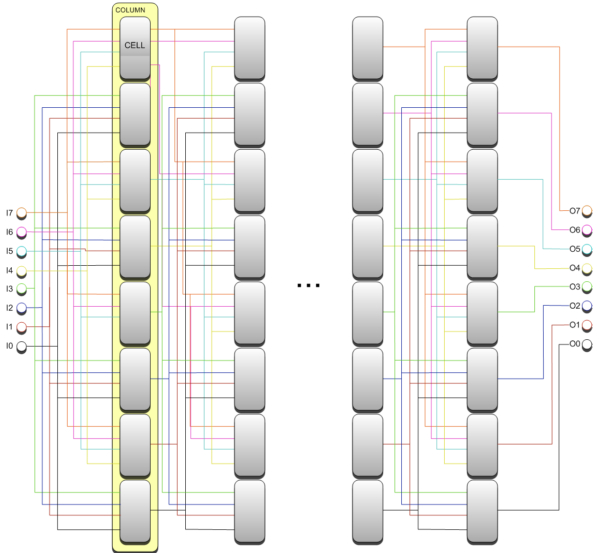
\includegraphics[width=\columnwidth]{Pictures/candidate.png}%
\caption{Internal structure of a Candidate Solution proposed in \cite{virtex4}}}%
\label{fig:candidate}%
\end{figure}

\subsubsection{Systolic array of PEs and Optimized DPR}
\label{sec:dpr}
Other than \cite{virtex4}, \cite{dpr} uses a systolic array of PEs. In this approach, each PE is a basic computation unit able to perform a single operation on the data take from their close neighbors. The architecture can be easily extended to any other processing purposes, since new PEs can be added to the library. In addition, PEs included in this library can be reused among applications. As can be seen in fig. \ref{fig:pe}, the size of the implemented structure is 4x4, but it can be completely and easily scaled. This DPR with elements relocation is carried out using a special HW block, the reconfiguration engine (RE).

\cite{dpr} describes an implementation of this RE. By storing only the body of the bitstream (cutting of the header and the tail), overclocking the FPGA by 2,5x and including internal memory (to avoid pasting the same configuration module in different positions of the architecture) the DPR is optimized. Due to this the reconfiguration time is greatly reduced. Adding the header and the tail of the bitstream at runtime has two additional advantages: it is allowed having a unique bitstream for each PE that can be configured in any position of the array. Also, bitstream reduction reduces the data transference time from the external memory.

% -- Plaatje systolic PE array architecture ---------------------------
\begin{figure}[htb]%
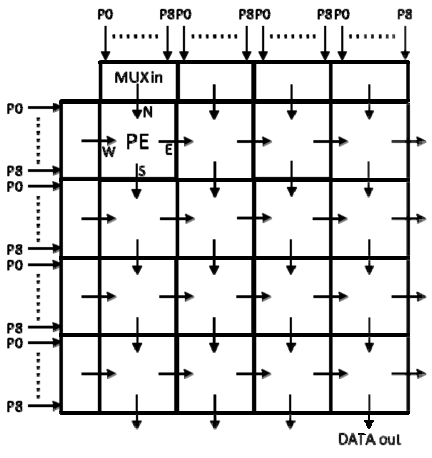
\includegraphics[width=\columnwidth]{Pictures/PE}%
\caption{Systolic array of PEs introduced by \cite{dpr}}%
\label{fig:pe}%
\end{figure}

\subsubsection{Erlangen Slot Machine}
The architecture of \cite{erlangen} the Erlangen Slot Machine (ESM) deals with the three drawbacks of FPGAs mentioned in \ref{sec:fpga}, being fixed pins which are spread around the device (I/O dilemma0, the inter-module dilemma and the local memory dilemma. 

First, the I/O dilemma caused by fixed pins spread around the device is solved by connecting all bottom pins from the FPGA to an interface controller realizing a crossbar, as can be seen in figure \ref{fig:erlangen}. It connects FPGA pins to peripherals automatically based on the slot position of a placed module. This I/O rerouting principle is done without reconfiguration of the crossbar FPGA.

Second, the memory dilemma has been solved. In normal Virtex-II FPGAs, a module can only occupy the memory inside its physical slot boundary. Storing data in off-chip memories is therefore the only solution. In the ESM, six SRAM banks are connected to the FPGA. Since these banks are placed at the opposite side as the crossbar, a module will connect to peripherals from one side, while the other side will be used for temporally storing computational data. In order to use a SRAM bank (called a slot), the module must have at least a width of three micro-slots, in which the total device is divided (see \ref{fig:erlangen}). This organization simplifies relocation, enabling a partially reconfigurable computing system. Also, equal resources will be available for each module.

Finally, the inter-module communication dilemma is dealt with. Dynamically routing signal lines on the hardware is a very difficult task. The ESM uses a combination of bus-macros, shared memory, RMB (Reconfigurable Multiple Bus) and a crossbar to take away the limiting factor for the wide use of partial dynamic reconfiguration (\cite{erlangen}).

% -- Plaatje ESM ---------------------------

\begin{figure}[htb]%
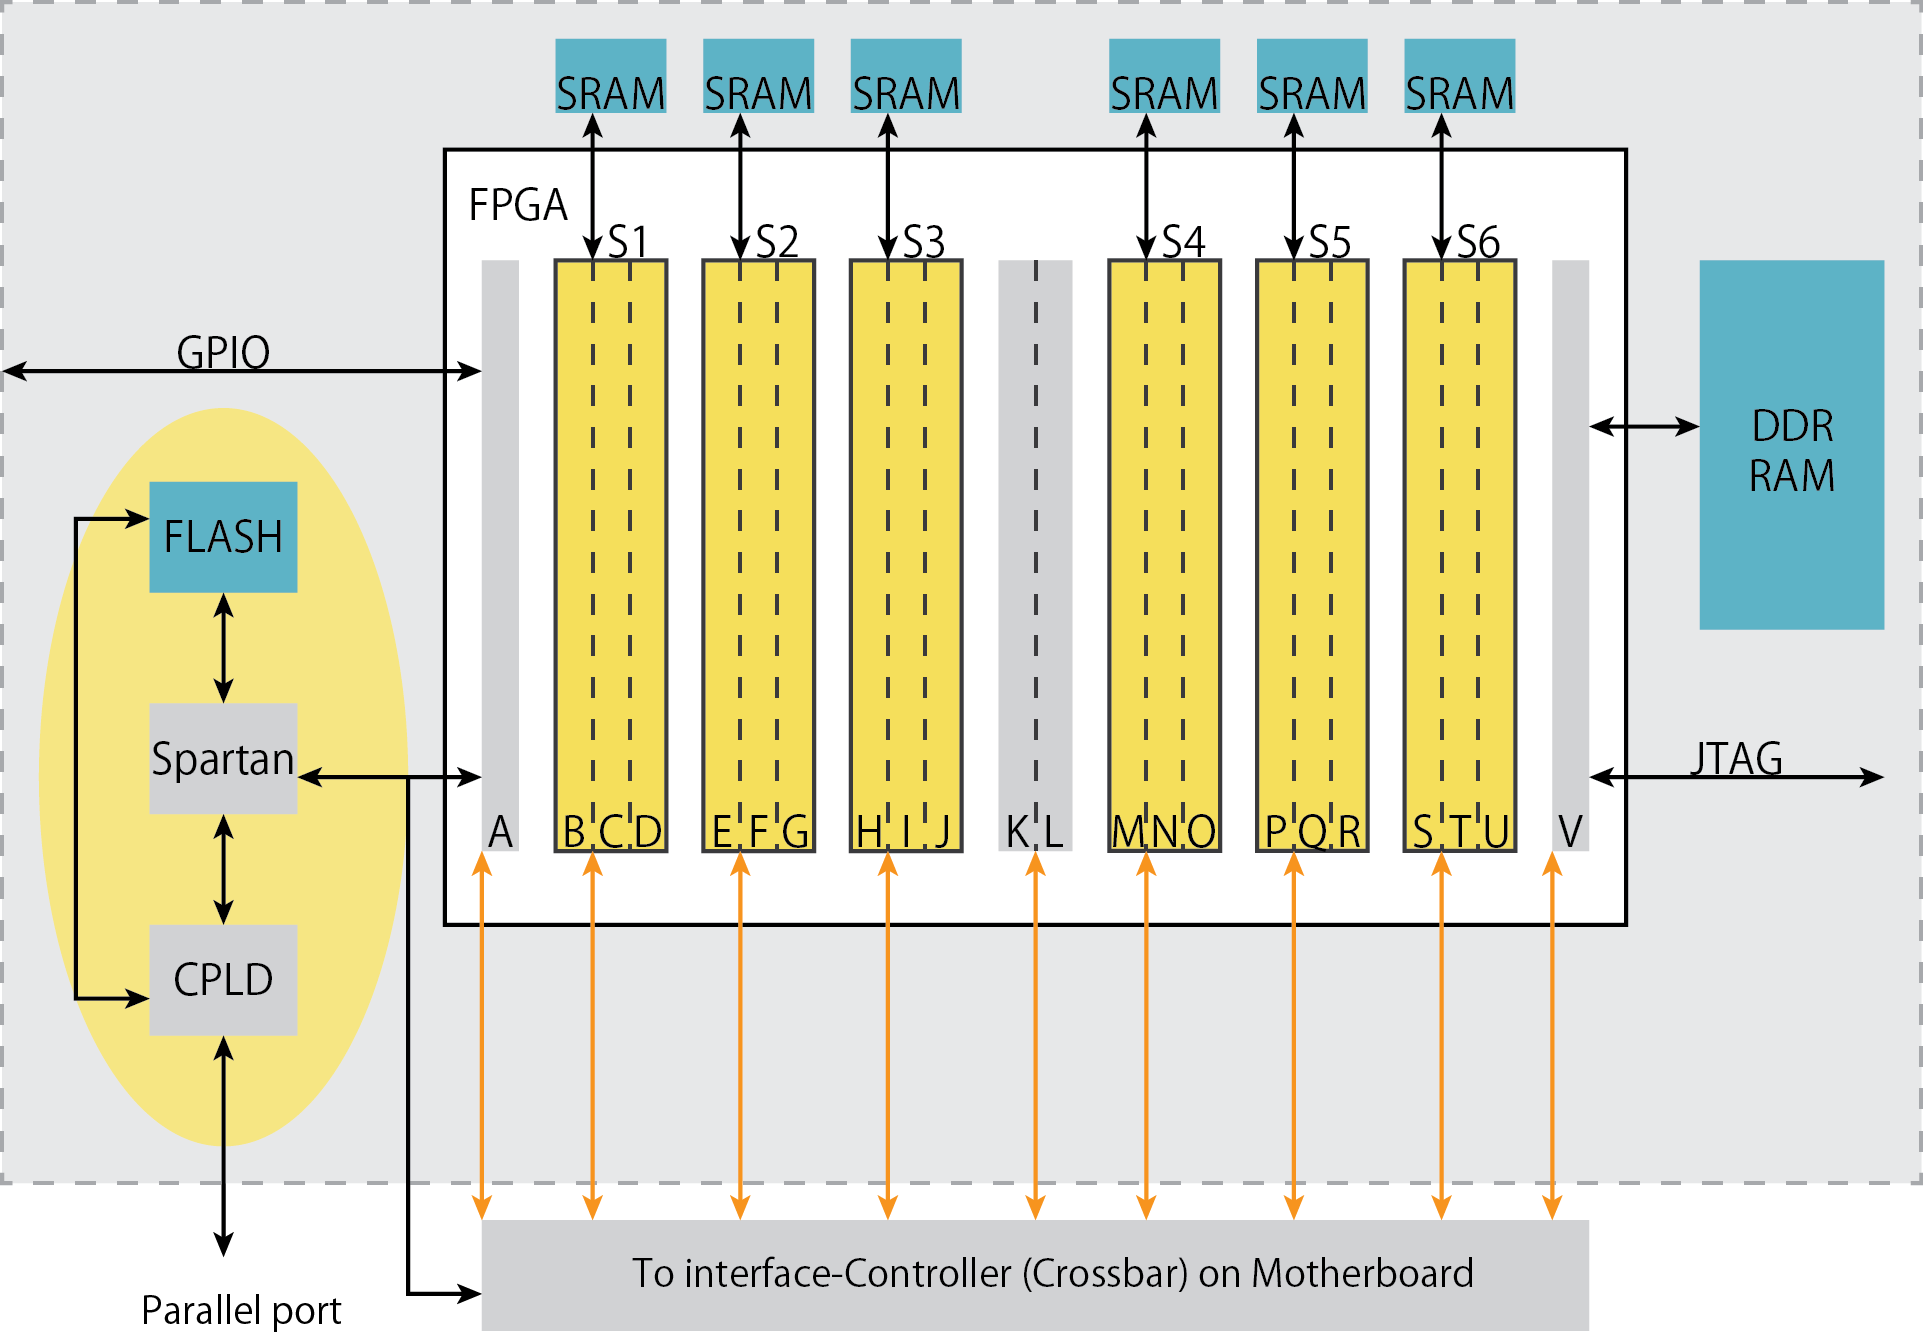
\includegraphics[width=\columnwidth]{Pictures/erlangen}%
\caption{Architecture of the ESM board. Three consecutive micro-slots define a macro-slot, which can access one full external SRAM bank.}%
\label{fig:erlangen}%
\end{figure}


% not important papers
%%Self-managed Systems: An Architectural Challenge

A self-managed software architecture is one in which component automatically configure their interaction in a way that is compatible with an overall architectural specification to achieve the goals of the system. Dynamic change which occurs while the system is operational, is far more demanding and requires the system to evolve dynamically and that adaption occurs at run-time. There is a community called SEAMS (Software engineering for adaptive and self-managing systems).

They focus on the use of ADLs for software design and implementation from components, including limited language support for dynamic change, a general model for dynamic change and evolution, associated analysis techniques and initial steps towards self-management.

The three-layer Gat model is presented. The bottom control layer consists of sensors, actuators and control loops and includes facilities to report the status to the middle layer. The change management layer, or middle layer reacts to state changes accordingly and can introduce new components. The upper goal layer consists of time consuming computations such as planning. They propose a component design that implements the set of services that it provides and the set that it may need.

		% May, 2007, not usefull, just for the intro
%% A New Architecture for Trustworthy Autonomic Systems

Validation alone does not always guarantee trustworthiness as each individual decision could be correct, but the overall system might not be consistent or dependable. These aspects should be integrated at architectural level and not be seen as add ons. Autonomic computing is mostly based on the architecture's basic MAPE (monitor, analyze, plan, execute) control loop. Another inspiration for autonomic systems is Intelligent Machine Design (IMD), based on the human autonomic nervous system.

In large systems with a wide behavioral space it is highly complex to determine whether all autonomic decision were in overall interest of the system. There is a vital need to dynamically validate the run-time decisions of the autonomic manager. The higher goal is not to just reach self-management, but to achieve consistency and reliability of results through self-management.

Current research has looked into a fifth state of the self* properties: self-regulation. It tests itself integral in the architectural, however it assumes that the other states perform optimally and they do not ensure trustworthiness. Another believe is that trustworthiness is achieved when keeping an account of its behavior. This requires the user to intervene if necessary. A dead-zone can be introduced to prevent unnecessary inefficient and ineffective control brevity when the system is sufficiently close to its target value.

The proposed trustworthy architecture exists out of  Autonomic Controller, an Validation Check, a Dependability Check and the managed sub-system. The AC doesn't matter about the content of the unit, but only provides an interface to the designers to express rules that govern the goal. The VC is a higher level mechanism that keeps track of the goal. It is important to also consider the possibility of overall inconsistency in the behavior of the system (the AM could erratically be changing its mind, causing oscillation). The DC only allows the AM to change its mind when its necessary and safe to do so.  Dead-zone logic is implemented to account for this, as well as prediction and learning. A system, no matter the context of deployment, is truly trustworthy when its actions are continuously validated to satisfy set requirements.
	% September, 2012

